\documentclass[11pt, a4paper]{article}

\usepackage[spanish]{babel}
\usepackage[utf8]{inputenc}
\usepackage{graphicx}
\usepackage{caption}
\usepackage{subcaption}

% Margin set to a4wide
\usepackage{geometry}
\usepackage{layout}

\geometry{
  left=2.5cm,
  right=2.5cm,
  top=3.5cm,
  bottom=3cm
}

\usepackage{amsmath}
\usepackage{amstext}
\usepackage{amssymb}
\usepackage{hyperref}

\linespread{1.3}

\title{
    \large{Computación Paralela: Trabajo Final}\\
    \huge{Similitud Coseno Punto a Punto}
}

\author{Cristian A. Cardellino}

\date{12 de Agosto de 2015}

\begin{document}
  \maketitle

  \section{Introducción}

  El presente informe describe el trabajo final realizado para la cátedra de
  posgrado ``Computación Paralela''. El proyecto elegido fue la paralelización
  del algoritmo de {\em similitud coseno punto a punto} (pairwise cosine
  similarity) de una matriz.
  
  A grandes rasgos, el algoritmo toma una matriz y compara cada fila de esta
  contra todas las demás filas utilizando similitud coseno entre los vectores
  conformados por las filas. Luego devuelve una matriz de distancia con las
  distancias de cada par de filas en la matriz.

  La similitud coseno es una medida de la similitud existente entre dos
  vectores, en un espacio vectorial que posee producto punto, con el que se
  evalúa el valor del coseno del ángulo comprendido entre ellos. Esta medida
  proporciona un valor igual a 1 si el ángulo es cero, es decir ambos vectores
  apuntan al mismo lugar. Ante cualquier ángulo existente entre los vectores la
  medida arrojaría un valor menor a uno. En caso de vectores ortogonales la
  similitud es nula. Finalmente, si los vectores son opuestos, la medida sería
  -1.

  La similitud coseno puede ser aplicada a varias dimensiones, y es más
  comúnmente utilizada en espacios de alta dimensionalidad, e.g. búsqueda y
  recuperación de información (information retrieval) o minería de textos (text
  mining). 

  La similitud punto a punto es utilizada como técnica en sistemas de
  recomendación (recommender systems), particularmente en filtrado colaborativo
  (collaborative filtering), donde una matriz representa valoraciones
  (ratings) que ciertos usuarios les dan a ciertos items y esto a su vez es
  utilizado para recomendar dichos items a otros usuarios basándose en la
  similitud que tienen valorando items.

  La paralelización del presente problema se da en que la similitud entre dos
  filas de la matriz es completamente independiente por cada par de filas que
  haya en la matriz. No obstante, realizar este trabajo secuencialmente es del
  orden $\mathcal{O}(n^{2})$, donde $n$ es la cantidad de filas de la matriz.

  El informe se estructura de la siguiente manera: en la
  Sección~\ref{sec:problema} se describe el problema particular sobre el que se
  trabajaron las técnicas de optimización, se presentan los datos utilizados y
  la manera en que se preprocesaron y como se representan dentro del problema;
  la Sección~\ref{sec:optimizaciones} describe los procesos que se llevaron a
  cabo buscando optimizar el problema con distintos procedimientos; la
  Sección~\ref{sec:resultados} muestra los resultados de los experimentos y
  hace un análisis general de los mismos; finalmente el reporte concluye en la
  Sección~\ref{sec:conclusiones}, donde se hace una observación general del
  problema y los objetivos alcanzados.
 
  \section{Descripción del problema, datos y representación}\label{sec:problema}

  \subsection{Filtrado colaborativo basado en items}

  Los sistemas de recomendación (recommender systems) buscan predecir las
  preferencias de ciertos usuarios sobre ciertos items. En los últimos años se
  ha visto que estos sistemas se volvieron extremadamente comunes en distintas
  áreas como libros, películas, música, y productos en general. Grandes
  jugadores del medio del e-commerce o que brindan servicios de streaming hacen
  uso de estos sistemas para brindar una mejor experiencia de usuario (Netflix,
  Amazon, Spotify, entre otros).

  Dentro de estos sistemas, una técnica muy utilizada es el filtrado
  colaborativo (collaborative filtering) cuya idea parte de que usuarios
  similares tendrán gustos similares. El filtrado colaborativo es un método que
  busca hacer predicciones automáticas (filtrado) sobre los intereses de un
  usuario recolectando las preferencias de varios usuarios. La suposición que
  hace esta técnica es que si un usuario {\it A} tiene una opinión similar a un
  usuario {\it B} sobre determinado asunto, {\it A} es más probable que tenga
  una opinión similar a {\it B} en un asunto diferente a que tenga una opinión
  similar a algún otro usuario aleatorio {\it C}. Esto también es conocido como
  {\em filtrado colaborativo basado en usuarios} (user-based collaborative
  filtering) y tiene algunos problemas como:

  \begin{itemize}
    \item Bajo desempeño cuando hay muchos items pero pocas calificaciones.
    \item La cantidad de usuarios suele sobrepasar por varias magnitudes al
        número de items.
    \item Las preferencias de los usuarios pueden cambiar, lo que implica tener
        que recalcular todo el sistema.
  \end{itemize}

  Una variante de la técnica de filtrado colaborativo llamada {\em filtrado
  colaborativo basado en items}~\cite{linden2001collaborative} (item-based
  collaborative filtering) fue patentada por Amazon, y resuelve la mayoría de
  los problemas presentados por el filtrado basado en usuarios, particularmente
  en sistemas donde hay más cantidad de usuarios que de items. La idea base de
  esta técnica es recomendar items que sean similares a otros items que el
  usuario ya calificó positivamente, midiendo la similitud de dichos items. En
  este proyecto se busca paralelizar y optimizar el código básico que se usa
  para hacer este filtrado colaborativo basado en items.

  \subsection{Datos utilizados}\label{sec:datos}

  Para el desarrollo del proyecto se optó por datos estándar en la
  investigación de algoritmos de recomendación:
  MovieLens~\cite{Harper:2015:MDH:2866565.2827872}, de GroupLens Research. Este
  consta de distintas valoraciones (ratings) que usuarios del sitio web
  MovieLens\footnote{\url{http://movielens.org}} hicieron sobre distintas
  películas.

  GroupLens liberó distintos tamaños de su conjunto de datos para
  investigación. En este trabajo se hace uso de 4 de ellos:

  \begin{description} 
      \item[MovieLens 100k Dataset (ML100k)] Consta de 100000 valoraciones
          realizadas por 943 usuarios sobre 1682 películas.
      \item[MovieLens 1M Dataset (ML1M)] Consta de 1000209 valoraciones
          realizadas por 6040 usuarios sobre 3962 películas.
      \item[MovieLens 10M Dataset (ML10M)] Consta de 10000054 valoraciones
          realizadas por 69878 usuarios sobre 10677 películas.
      \item[MovieLens 20M Dataset (ML20M)] Consta de 20000263 valoraciones
          realizadas por 138493 usuarios sobre 26744 películas.
  \end{description}

  Las valoraciones de los usuarios están hechas en una escala de 5 estrellas
  (i.e. del rango [1, 5]), que en el caso de los datos de ML10M y ML20M pueden
  tener incrementos de media estrella (i.e., en el rango [0.5, 5.0]). Todos los
  conjuntos establecen que cada usuario valoró un mínimo de 20 películas.

  Los conjuntos ML100k y ML1M no tuvieron que ser modificados debido a que
  estos identificaron a sus películas y usuarios unívocamente con la cantidad.
  En el caso de los conjuntos ML10M y ML20M, estos tenían a sus usuarios y
  películas identificados con más números que la cantidad, por lo que se los
  preprocesó proyectando los valores de manera que estos fueran unívocos a la
  cantidad de usuarios/películas.

  \subsection{Representación de los datos}\label{sec:representaciones}

  Se requiere de dos archivos para hacer funcionar el código: la matriz de
  valoraciones y la matriz de similitud para corrección. La primera se obtuvo a
  partir de los datos brindados por MovieLens, la segunda se calculó utilizando
  la librería de aprendizaje automático de Python ``Scikit
  Learn''~\cite{scikit-learn}.

  La matriz de valoraciones contiene una fila por cada película y una columna
  por cada usuario del conjunto de datos.  Cada celda de la matriz representa
  la cantidad de estrellas que el usuario le dio a la película, siendo este
  valor igual a cero cuando el usuario no hizo valoración alguna sobre dicha
  película.

  Debido a que el conjunto de datos establece que cada usuario valoró un mínimo
  de 20 películas, dejando la mayoría de las películas sin valorar, la matriz
  final de películas/usuarios es extremadamente rala, llegando a ser los
  valores no nulos menor al 1\% de la totalidad de la matriz.

  En los primeros experimentos la matriz películas/usuarios era representada
  por una matriz densa. Sin embargo, era solo viable para los casos de los
  conjuntos ML100k y ML1M que se podía cargar dicha matriz en memoria sin que
  afectara gravemente el desempeño de los algoritmos encargados de calcular la
  similitud coseno. Buscando mejorar este desempeño para conjuntos de datos de
  mayor tamaño se optó por el uso de representaciones ralas para matrices; y
  dado que se necesita un acceso rápido a las filas para su comparación se hace
  uso del formato Yale (o {\em compressed row storage}) para representar las
  matrices.
  
  El archivo con el que se guarda la matriz de valoraciones sigue la base del
  formato de intercambio {\em Matrix Market}~\cite{Boisvert:aa}. Se usa el
  formato COO de matrices ralas coordinadas que durante la etapa de carga se
  transforma en formato Yale. 

  La matriz de corrección tiene la particularidad de ser una {\em matriz de
  distancia}, lo que quiere decir que es simétrica a través de la diagonal
  principal. Por lo tanto es suficiente con guardar la mitad triangular
  superior de la matriz. Para esto se hace uso de la propuesta de James D.
  McCaffrey: ``Converting a Triangular Matrix to an
  Array''\footnote{\url{https://jamesmccaffrey.wordpress.com/2010/05/14/converting-a-triangular-matrix-to-an-array/}}.

  \section{Optimizaciones}\label{sec:optimizaciones}

  \subsection{Algoritmo Base}

  El primer algoritmo, sin ninguna clase de optimización, es el que se busca
  mejorar en las instancias sucesivas de optimización.

  El algoritmo comienza por cargar la matriz de ratings en su versión COO
  dentro de un arreglo utilizado como matriz de N filas por 3 columnas, donde N
  es el número de datos (en este caso ratings que posee el dataset) y en las 3
  columnas se almacena el valor de la fila (el ID de la película), el valor de
  la columna (el ID del usuario) y el rating. Esta es una representación
  sencilla de una matriz rala en formato COO.

  Si bien originalmente esta matriz era de enteros puesto que en los dos
  conjuntos de datos de menor tamaño (ml100k y ml1M, como se describe en la
  Sección~\ref{sec:datos}) los ratings eran únicamente valores enteros entre 1 y
  5. Sin embargo para los dos conjuntos de datos de mayor tamaño, los ratings
  podían tener ``media estrella'', por lo que los valores ya podían ser
  flotantes. Por esta razón, el arreglo pasó a ser de flotantes. 

  Se continúa con la carga del vector de corrección, que viene a ser el vector
  que representa la matriz de similitud coseno (como se describe en la
  Sección~\ref{sec:representaciones}) y que sirve como {\em gold standard} para
  asegurarse de que los cálculos se hicieron bien.

  El paso final de carga es el de la matriz de valoraciones, también descripta
  en la Sección~\ref{sec:representaciones}.  Esta será la matriz que se
  utilizará como base para los cálculos que se buscan optimizar. En los
  primeros experimentos esta matriz tiene una representación densa (a pesar de
  ser extremadamente rala).

  El algoritmo que se encarga del cálculo de la matriz de similitud coseno toma
  como entrada la matriz de valoraciones. El cálculo se realiza recorriendo
  cada par de filas (películas) una vez (puesto que la similitud entre la fila
  {\em i} y la fila {\em j} es la misma que la similitud entre la fila {\em j}
  y la fila {\em i}) y aplicando la {\em similitud coseno} entre los dos
  vectores que forman el par de filas.  En total, para recorrer todos los pares
  de filas de la matriz de valoraciones se necesitan
  $\frac{\text{P}^2+\text{P}}{2}$ iteraciones, donde P es el número de
  películas (o filas) de la matriz de valoraciones. Este valor es la dimensión
  final del vector que representa la matriz de similitud.

  La similitud coseno entre dos vectores \textbf{U} y \textbf{V} se define
  como:

  \[
      \text{cos\_sim}(\mathbf{U}, \mathbf{V}) = {\frac{\mathbf{U}\cdot\mathbf{V}}{\|\mathbf{U}\|\|\mathbf{V}\|}} = 
      {\frac {\sum \limits _{i=1}^{n}{U_{i}V_{i}}}{{\sqrt {\sum \limits _{i=1}^{n}{U_{i}^{2}}}}
      {\sqrt {\sum \limits _{i=1}^{n}{V_{i}^{2}}}}}}
  \]

  La sumatoria del numerador (num), la sumatoria del denominador para el vector
  \textbf{U} (uden), y la sumatoria del denominador para el vector \textbf{V}
  (vden), se realizan en el bucle que recorre cada par de filas. Luego, al
  final se almacena el valor de la similitud coseno dividiendo {\em num} por
  las raíces cuadradas de {\em uden} y {\em vden}. Este procedimiento se
  repite durante algunas iteraciones para eliminar el ruido proveniente del uso
  de CPU para el cálculo. 

  El algoritmo finalmente compara la matriz de similitud (almacenada como un
  vector como se describe en la Sección~\ref{sec:representaciones}) con el
  vector de corrección cargado previamente.

  Por obvias razones este algoritmo es lento y se hace más y más difícil llegar
  a un resultado a medida que el tamaño del problema incrementa. Las primeras
  optimizaciones que se intentaron son con el uso de flags del compilador. No
  obstante sólo se probó el desempeño sin optimizaciones del compilador
  únicamente en el caso del conjunto de datos de menor tamaño (ml100k), puesto
  que cualquiera de los otros conjuntos hubieran terminado luego de demasiado
  tiempo y no aportarían nada al presente trabajo. Sólo las optimizaciones de
  compilación mejoraron el desempeño en aproximadamente {\bf 2.18x}.

  Hacer único el recorrido de cada par de filas fue también una mejora (obvia
  de realizar) con respecto a los primeros algoritmos donde se recorría cada
  par de filas existentes y no se discriminaban aquellos pares cuya conmutación
  había sido ya calculada. Además, en las primeras instancias también se
  utilizó una matriz densa para guardar los resultados de la matriz de
  similitud, lo que hacía que se duplicara la cantidad de valores a guardar
  (además de la memoria necesaria para estos).

  \subsection{OpenMP}

  Una optimización bastante sencilla de realizar sobre el cálculo en CPU era la
  paralelización en threads mediante OpenMP de los bucles que se encargan de
  recorrer los pares de filas de la matriz.

  Dado que cada par de filas posee una similitud coseno independiente de los
  demás pares y como cada par se recorre una sola vez (discriminando la
  conmutación de filas), esto era trivialmente paralelizable mediante el uso de
  un decorador \texttt{pragma omp parallel for}. Esto probó mejorar el
  desempeño en gran medida respecto a la versión base del algoritmo. Por
  supuesto, mientras más threads se usen, más rápido se obtienen los
  resultados.

  Como existen dos bucles anidados que recorren la matriz (necesario para
  recorrer cada par de filas de la misma), se probó con la paralelización
  únicamente del bloque externo así como con la paralelización de ambos
  bloques. Esto fue también para ver si de una u otra manera el problema
  escalaba mejor. No obstante los resultados para uno u otro método fueron los
  mismos por lo que se decidió realizar las mediciones siguientes sólo
  utilizando un bucle paralelizado.

  \subsection{CUDA}\label{sec:optimizacion:cuda}

  La siguiente optimización que se buscó sobre los cálculos fue mediante el uso
  de CUDA para paralelizar los cálculos vía GPU. La base para cargar las
  matrices y vectores es la misma que en el caso de CPU. Por la naturaleza de
  CUDA, también hay que reservar los recursos necesarios en la GPU, además de
  hacer el traspaso de los datos desde la memoria del host a la memoria del
  device, lo que suma tiempo de cómputo.

  En CUDA, los kernels que se corren en paralelo son los encargados de un solo
  par de filas (películas) de la matriz. Se asegura mediante guardas
  condicionales que esto sea así para evitar condiciones de carrera. El
  algoritmo para hacer el cálculo es el mismo que en el caso que no se hace uso
  de GPUs, con algunas modificaciones como por ejemplo hacer uso de la función
  \texttt{rsqrt} para obtener las recíprocas de las raíces de los
  denominadores.

  Dado que necesitamos dos variables distintas en CUDA para recorrer la matriz
  (una por cada fila del par), los bloques de threads y del grid deben ser
  bidimensionales. De esta manera, una dimensión se utiliza para identificar
  unívocamente una fila del par, mientras que la otra dimensión se utiliza para
  identificar la otra fila del par. Por esta razón, cada dimensión de los
  bloques no puede poseer más de 32 threads (de lo contrario sería de un total
  superior a 1024 threads por bloque). El tamaño de ambas dimensiones de la
  grilla, a su vez, se calcula de manera tal que se puedan procesar todas las
  filas de la matriz de similitud.

  CUDA muestra una mejora importante en los tiempos de cálculo con respecto a
  la paralelización vía GPU. Sin embargo, hay que destacar que el tiempo extra
  que le toma a CUDA toda la configuración previa al cálculo suma bastante al
  resultado final, especialmente para los conjuntos de datos más pequeños, al
  punto de ser más lento para el caso particular del conjunto de datos ml100k.
  El peso del tiempo de configuración disminuye a medida que el tamaño del
  problema se hace mayor.

  \subsection{Matrices Ralas}

  La optimización final que se realiza sobre el problema original, y también la
  definitiva, es reemplazar la matriz de valoraciones por una representación
  rala de la misma. Esto mejora la performance tanto en velocidad como en
  memoria consumida.
  
  Dado que se busca realizar comparaciones por cada par de filas de la matriz,
  la mejor opción de representación de una matriz rala se encuentra en el
  formato Yale, también conocido como formato CRS (o Compressed Row Storage).
  La matriz se carga directamente desde el formato COO (que es con el formato
  que es guardada), al formato CRS, lo que elimina el proceso de convertir COO
  a una matriz densa. Si bien CUDA posee una librería para el manejo de
  matrices ralas, se optó, por simplicidad, por una representación simple
  mediante una estructura de datos nativa que hiciera uso de arrays para
  guardar los valores no nulos, índices, punteros y el tamaño de la matriz
  rala.

  Para esta representación se tuvo que replantear la manera en que se calculaba
  la similitud coseno entre dos filas, puesto que la forma para matrices densas
  no funciona dado que no todas las filas tienen las mismas columnas para la
  representación rala de la matriz.

  En lugar de calcular el numerador y los denominadores en un mismo bucle
  \texttt{for}, se hace uso de tres bucles distintos: un bucle \texttt{while}
  para el cálculo del numerador y dos bucles \texttt{for} por separado para el
  caso de los denominadores. Esta fue la manera de evitar tener que pasar por
  muchas columnas en cada fila cuyos valores eran cero y no aportaban nada al
  resultado final.

  El caso del primer bucle, se optó por \texttt{while} porque era la forma de
  mantener control sobre que columna (o bien índice) de la fila se estaba
  realizando la operación de sumatoria. Y como esta es en sí un producto punto
  entre dos vectores ralos, solo tiene sentido que se sumen aquellos índices
  cuyo valor es distinto de cero.  Para el caso de los denominadores, se
  resolvió el cálculo por separado de cada denominador para sólo tener que
  recorrer las columnas en las que dicho denominador tenía valores no nulos.

  El valor final de la matriz de similitud sí se calcula de la misma manera que
  en los algoritmos anteriores.

  \section{Análisis de resultados}\label{sec:resultados}

  \subsection{Recursos de hardware}

  Se utilizó zx81 para realizar las mediciones de desempeño. El siguiente
  cuadro detalla los recursos de hardware de los que se dispusieron.

  \begin{table}[h]
      \centering
      \begin{tabular}{ll}
          \hline
          \textbf{CPU} & Intel(R) Xeon(R) CPU E5-2620 \\
          \textbf{Frecuencia} & 2.40 GHz \\
          \textbf{Cores} & 12 \\
          \textbf{Memoria} & 126 GiB \\
          \textbf{GPU} & NVIDIA GeForce GTX Titan \\
          \textbf{Memoria GPU} & 12 GiB \\
          \hline
      \end{tabular}
      \caption*{Recursos de hardware}
  \end{table}

  Cabe destacar que la GPU utilizada posee una velocidad muy superior en
  problemas de precisión simple y que las mediciones fueron realizadas en doble
  precisión. Precisión simple puede llegar a ser suficiente para el tipo de
  problema que nos concierne y queda como trabajo futuro la correcta medición
  de los mejores algoritmos (i.e., matrices ralas) en precisión simple o bien
  en una placa cuya doble precisión sea más rápida.
 
  \subsection{Resultados}

  \subsubsection{Experimentos con OpenMP}

  \begin{figure}[ht]
    \centering
    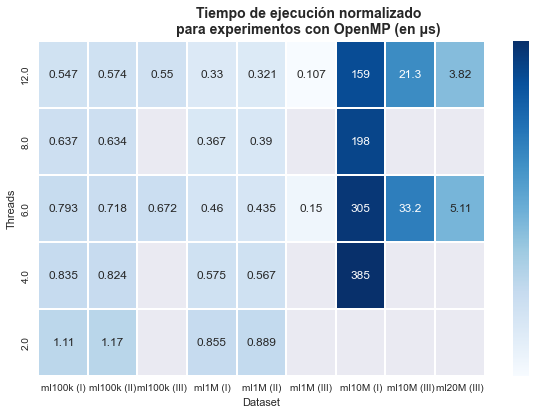
\includegraphics[width=\textwidth]{plots/heatmap_openmp.png}
      \caption{Heatmap de experimentos usando OpenMP}\label{fig:heatmap:omp}
  \end{figure}
 
  Se realizaron varios experimentos haciendo uso de OpenMP para el cálculo de
  los datos. Para ver la escalabilidad de la paralelización con threads vía
  CPU se probó realizar los experimentos con distinto número de threads.

  La Figura~\ref{fig:heatmap:omp} muestra los tiempos normalizados completos en
  microsegundos (i.e., el tiempo de cálculo sumado al tiempo de configuración)
  de distintos experimentos sobre los distintos conjuntos de datos, variando el
  número de threads con los cuales se corre OpenMP. Los tipos de experimentos
  que se detallan en la figura son los siguientes:

  \begin{itemize}
      \item Ejecución con uso de matrices densas: ml100k (I), ml1M (I),
          ml10M(I).
      \item Ejecución con uso de matrices ralas: ml100k (II), ml1M (II),
          ml10M (II), ml20M (II).
  \end{itemize}

  Como puede observarse, sólo en ``ml100k (I)'' y ``ml1M (I)'' se experimentó
  con 2, 4, 6, 8 y 12 threads. Por su lado ``ml10M (I)'', sólo usa a partir de
  4 threads, esto es así porque este conjunto de datos es mucho más grande que
  los conjuntos anteriores y hacerlo de menos de 4 threads hubiese tomado mucho
  tiempo de cómputo (que en el caso de CPU es más tendiente a generar errores
  por lo que se necesitan varias corridas lo que hace aún más lento el
  proceso). Por su parte no existe un ``ml20M (I)'' porque el conjunto de datos
  es demasiado grande como para poder levantarse en memoria utilizando una
  matriz densa de valoraciones, por lo que los únicos experimentos que pudieron
  hacerse sobre este conjunto fueron con matrices ralas.

  Como puede observarse, en los dos conjuntos de menor tamaño, la escalabilidad
  no es la deseada. Sin embargo, hay que tener en cuenta que en estos el peso
  del tiempo de configuración sobre el tiempo final es mayor que sobre los
  conjuntos de datos más grandes. En el caso de ``ml10M (I)'' se ve una
  escalabilidad mucho mejor duplicando el número de cores y siguiendo este
  patrón, lo más probable es que esto también fuera así para ml20M aplicado
  sobre matrices densas (suponiendo una cantidad de memoria lo suficientemente
  grande como para soportar dicha matriz. Esto es así porque en estos casos el
  tiempo de cómputo es casi la totalidad del tiempo final y el tiempo de
  configuración se vuelve despreciable.

  En los experimentos con matrices ralas se optó, por una cuestión de
  practicidad y tiempo, sólo ver si había escalabilidad en el paso de 6 a 12
  threads. Claramente esto no es así. Sin embargo, hay que tener en cuenta que
  matrices ralas ofrece otro tipo de desafíos extras en la algoritmia que por
  falta de tiempo no pudieron ser analizados más en profundidad.

  \subsubsection{Comparación de experimentos CUDA y OpenMP}
  
  \begin{figure}[ht]
    \centering
    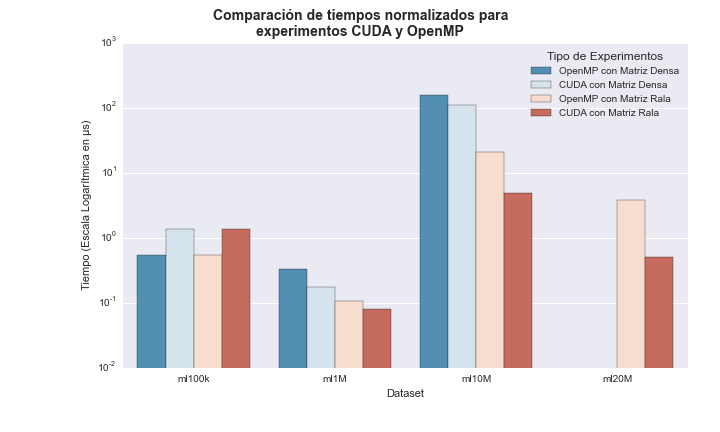
\includegraphics[width=\textwidth]{plots/cuda_omp.png}
      \caption{Comparación de experimentos CUDA y OpenMP}\label{fig:bar:cuda:omp}
  \end{figure}

  La Figura~\ref{fig:bar:cuda:omp} muestra la comparación de desempeño entre
  OpenMP y CUDA, utilizando matrices de valoración densas (barras de tonos
  azul) y ralas (barras de tonos rojizos). Los tiempos están normalizados de
  acuerdo al tamaño del problema y representan la suma entre tiempo de cálculo
  y tiempo de configuración. Los experimentos que hacen uso de OpenMP y
  paralelización vía CPU son corridos con 12 threads, mientras que todos los
  experimentos de CUDA corren un un tamaño de 32x32 threads por bloque (i.e.
  1024 en total).

  Se hacen mediciones por cada uno de los conjuntos de datos y como se puede
  ver, en general los algoritmos que hacen uso de matrices ralas son mejores
  que sus contrapartes que hacen uso de matrices densas. Esto implica una
  ganancia doble con este tipo de algoritmos: en memoria y en velocidad de
  cómputo. Un dato, resultado del uso de matrices ralas, es, como se explicó
  previamente, que el conjunto de datos de mayor tamaño (ml20M) no pudo ser
  ejecutado haciendo uso de matrices densas porque no cabía en memoria (en una
  máquina con > 120 GiB de RAM). Por otro lado, el conjunto de datos ml10M, el
  siguiente en tamaño, ocupa 6.2 GiB de memoria utilizando matrices densas,
  mientras que su tamaño es de 659 MiB haciendo uso de matrices ralas.

  El único caso donde no se ve tanto la mejora de matrices ralas sobre matrices
  densas (y particularmente de CUDA sobre OpenMP) es en el conjunto de menor
  tamaño: ml100k. Como se dijo estos tiempos no son sólo los de cómputo sino
  que también se consideran los tiempos de configuración, algo que pesa más en
  conjuntos de datos de menor tamaño.

  \subsubsection{Experimentos con CUDA}

  \begin{figure}[ht]
    \centering
    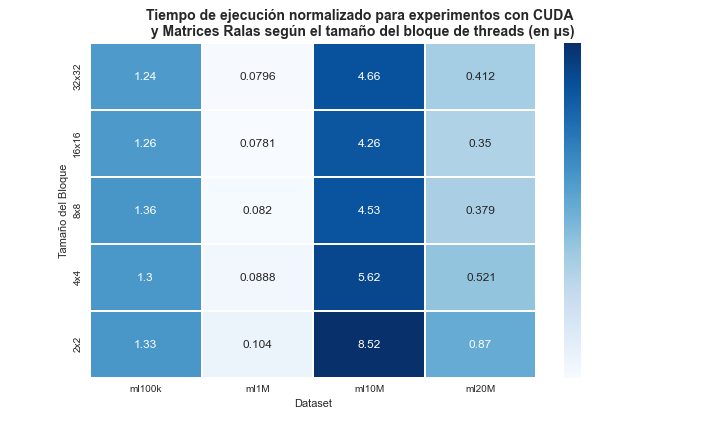
\includegraphics[width=\textwidth]{plots/cuda_sparse_blocks.png}
      \caption{Heatmap de experimentos usando CUDA}\label{fig:heatmap:cuda}
  \end{figure}

  Una vez determinado que matrices ralas con CUDA prueban estar entre los
  mejores resultados en general, se comparó el desempeño del algoritmo con
  distinta cantidad de threads por bloque. La Figura~\ref{fig:heatmap:cuda}
  muestra los distintos tiempos normalizados en microsegundos de los
  experimentos realizados.

  Se recuerda que, por la naturaleza del problema y la necesidad de recorrer
  dos dimensiones distintas en la matriz como se explicó en la
  Sección~\ref{sec:optimizacion:cuda}, el tamaño del bloque es necesariamente
  un cuadrado perfecto (y en este caso una potencia de 2), luego, se probó con
  las siguientes cantidades de threads por bloque: $32\times32=1024$,
  $16\times16=256$, $8\times8=64$, $4\times4=16$, $2\times2=4$.

  Como puede observarse, no hay gran variación en el tiempo, sobre todo a
  partir de $4\times4$ threads por bloque. Y en general un bloque de
  $16\times16$ arroja los mejores resultados en casi todos los conjuntos de
  datos; siendo ml100k la única excepción con un error de $2\mathrm{e}{-2}$,
  que probablemente sea despreciable sobre todo si se trata del tiempo extra
  para configuración que en este caso tiene más peso que en los otros.

  \subsubsection{Evolución en los distintos experimentos}

  Se presenta a continuación la evolución para los 4 conjuntos de datos
  utilizando para cada uno distintos puntos en el proceso de optimización que
  muestran la evolución en la mejora del tiempo a lo largo de los distintos
  experimentos.

  \begin{figure}[ht]
      \centering
      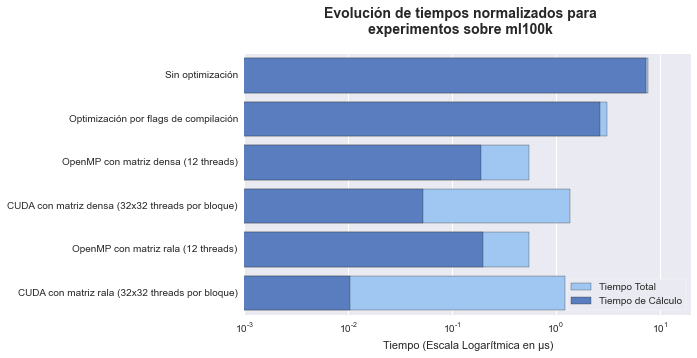
\includegraphics[width=\textwidth]{plots/ml100k.png}
      \caption{Evolución de tiempos sobre ml100k}\label{fig:ml100k}
  \end{figure}

  La Figura~\ref{fig:ml100k} muestra los resultados para el conjunto de datos
  más chico: ml100k. Este conjunto de datos, por obvias razones, fue sobre el
  que más experimentos se realizaron. En este, y todos los gráficos de la
  sección, se muestran los distintos tiempos normalizados en microsegundos
  (tener en cuenta que también se muestran los resultados en escala
  logarítmica). También, los gráficos destacan el tiempo total y la fracción
  de ese tiempo que tomaron los cálculos.

  El gráfico muestra como primer hito el tiempo sin realizar ninguna
  optimización, ni siquiera mediante flags de compilador. Se continúa con la
  optimización por flags de compilación: luego de probar distintos flags se
  determinó que \texttt{-O3} y el uso de {\em hugepages} daban las mejores
  mediciones, con una ganancia de {\bf 2.77x} respecto al problema sin
  optimización.

  Continuamos con OpenMP con matrices densas, que junto con la versión OpenMP
  con matrices ralas, obtienen los mejores tiempos para este conjunto de datos
  (tanto los el tiempo de cálculo como el tiempo total es similar en ambas
  versiones), con una mejora aproximada de {\bf 4.85x} sobre la optimización
  mediante flags de compilación y una mejora aproximada de {\bf 2.49x} sobre la
  versión CUDA con matrices densas y una mejora aproximada de {\bf 2.25x} sobre
  la versión CUDA con matrices ralas. Se observa no obstante como en este caso
  el peso de la configuración para correr CUDA modifica el resultado final de
  manera importante, dado que el tiempo de cálculo sigue siendo mejor en ambas
  versiones CUDA: para el caso de CUDA con matrices densas, los cálculos son
  3.6x más rápidos mientras que con el uso de matrices ralas la optimización
  escala a 18x.
 
  \begin{figure}[ht]
      \centering
      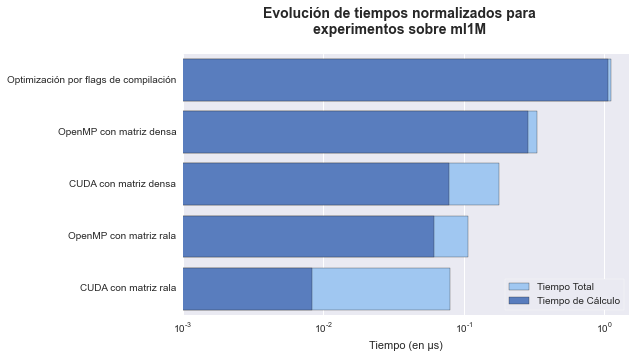
\includegraphics[width=\textwidth]{plots/ml1M.png}
      \caption{Evolución de tiempos sobre ml1M}\label{fig:ml1M}
  \end{figure}

  En segunda instancia tenemos la Figura~\ref{fig:ml1M} que muestra la
  evolución de las mediciones sobre el conjunto de datos ml1M. Arrancamos desde
  la optimización sólo por flags de compilación (pues no se midió sin
  optimización por considerarlo no relevante) y al pasar a la paralelización
  mediante OpenMP con matrices densas obtenemos una mejora aproximada de {\bf
  3.35x}. CUDA con matrices densas sigue mejorando los resultados en
  aproximadamente {\bf 1.87x}. Continúa OpenMP con matrices ralas que tiene una
  mejora sobre la versión CUDA con matrices densas de {\bf 1.65x} y finalmente
  las mejores mediciones quedan en la versión CUDA con matrices ralas,
  obteniendo una mejora sobre OpenMP con matrices ralas de {\bf 1.37x}.

  Como se observa, a medida que el tamaño del conjunto de datos aumenta,
  disminuye el peso del tiempo de configuración sobre el resultado final. Sin
  embargo sigue siendo importante, sobre todo para la mejor versión de CUDA,
  cuyo tiempo de cálculo es muy superior a la mejor versión de OpenMP.

  Es de destacar que los tiempos normalizados de este conjunto de datos en
  particular probaron ser los mejores entre todas las mediciones. Se necesita
  de un análisis más profundo de los datos para poder explicar este
  comportamiento que no se hará en este trabajo por razones de tiempo.
 
  \begin{figure}[ht]
      \centering
      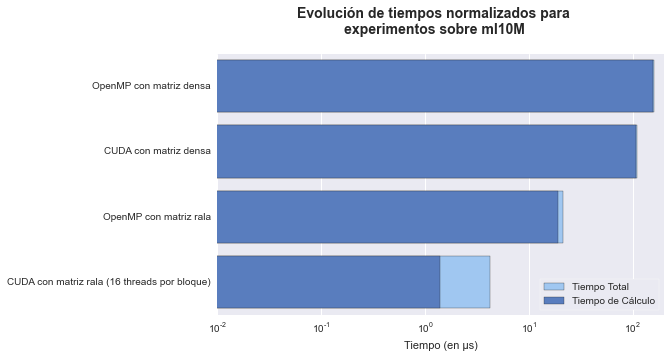
\includegraphics[width=\textwidth]{plots/ml10M.png}
      \caption{Evolución de tiempos sobre ml10M}\label{fig:ml10M}
  \end{figure}

  La Figura~\ref{fig:ml10M} muestra algunos de los resultados para el conjunto
  de datos ml10M. En este caso no se hicieron mediciones sin ningún tipo de
  paralelización porque el conjunto era demasiado grande como para hacerlo. Por
  lo tanto se tomaron medidas directamente sobre la paralelización vía CPU con
  OpenMP (y 12 threads) utilizando matrices densas como base.  El método CUDA
  con matrices densas ya obtiene una mejora de los resultados de
  aproximadamente {\bf 1.43x} sobre la versión OpenMP. De la misma manera, la
  versión OpenMP con matrices ralas mejora sobre la versión CUDA anterior en
  {\bf 5.22x}. Finalmente, la mejor versión, CUDA con matrices ralas, genera
  una mejora de aproximadamente {\bf 5x} sobre la versión OpenMP con matrices
  ralas.

  En este conjunto de datos se puede apreciar como el tiempo de configuración
  se va haciendo cada vez menos importante en el resultado final, afectando en
  mayor medida a la versión CUDA con matrices ralas y siendo prácticamente
  despreciable para las demás versiones del algoritmo.

  Como contrapartida al conjunto de datos anterior, este provee las peores
  mediciones normalizadas. Nuevamente, requiere un estudio más profundo de los
  datos para determinar que puede ser el causante de este comportamiento que se
  evitará hacer en el presente trabajo.
 
  \begin{figure}[ht]
      \centering
      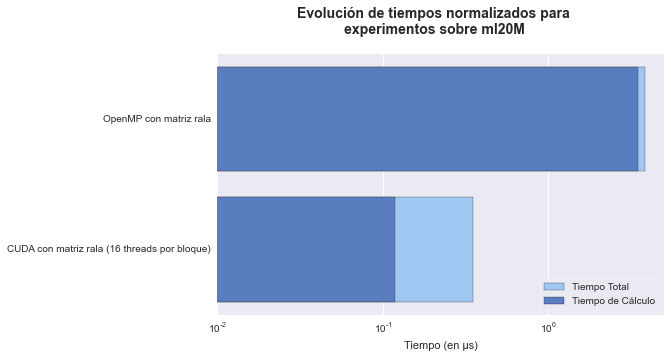
\includegraphics[width=\textwidth]{plots/ml20M.png}
      \caption{Evolución de tiempos sobre ml20M}\label{fig:ml20M}
  \end{figure}

  El último gráfico, presente en la Figura~\ref{fig:ml20M}, muestra los
  resultados sobre el conjunto de datos de mayor tamaño: ml20M. Como se explicó
  en previas secciones, para este conjunto de datos solo se pudo experimentar
  haciendo uso de matrices ralas debido a la inmensidad del conjunto. Se
  compara el uso de paralelización vía CPU con OpenMP contra la paralelización
  vía GPU con CUDA, siendo esta última la más veloz, con una ganancia de
  aproximadamente {\bf 10.91x}. Como en el caso del conjunto de datos anterior,
  se observa también que el tiempo de configuración tiene menos peso en el
  valor final de la medición y también que es mucho más importante para el caso
  de CUDA que para OpenMP, consecuencia del movimiento de datos entre la
  máquina anfitrión y el dispositivo.

  \section{Conclusiones}\label{sec:conclusiones}

  En este trabajo se realizó la optimización desde cero del código necesario
  para hacer cálculo de similitud coseno punto a punto en matrices de
  valoraciones. Algo muy utilizado para realizar filtrado colaborativo en
  sistemas de recomendación.  El trabajo hace uso de conjuntos de datos que son
  estándares clásicos en el estudio de sistemas de recomendación: los datos de
  MovieLens.

  A lo largo del trabajo se explican los diferentes procedimientos para lograr
  paralelizar el código, obteniendo mejores tiempos de cómputo finales.
  Comenzando con paralelización vía CPU con OpenMP y avanzando al uso de
  kernels CUDA y paralelización vía GPU.

  Si bien la paralelización ofrece tiempos de cómputo decentes y buenas
  mediciones en general, por la naturaleza del problema, se determinó que es el
  uso de matrices ralas, que representan mejor datos tan dispersos como las
  valoraciones que ciertas personas les dan a ciertos elementos, es lo que
  verdaderamente ofrece una diferencia. Esto se ve en particular para el caso
  de los conjuntos de datos más grandes, donde el uso de la matriz rala puede
  hacer la diferencia entre poder realizar estos cálculos o no: el conjunto
  ml20M ofrece un ejemplo perfecto de un problema que el uso de las estructuras
  correctas hace la diferencia entre poder o no realizar las operaciones.

  Este es un trabajo claramente introductorio al problema y que ofrece varios
  aspectos extras para explorar y mejorar. Uno de estos aspectos, de los más
  importantes, es la medición con el uso de precisión simple para ver su
  diferencia con precisión doble. También requiere un trabajo más cercano sobre
  los datos para determinar que hace que algunos conjuntos de datos posean
  mediciones normalizadas mucho mejores que otros. Finalmente, se debería hacer
  una exploración más cercana de la literatura que versa del tema para ver si
  el uso de estructuras especializadas (como aquellas que pueden ofrecer
  librerías como {\em cusparse}) mejora el rendimiento de manera significativa.
  Quedan estos temas como trabajo futuro sobre el problema.

  A grandes rasgos se lograron resultados satisfactorios y una mejora
  importante sobre un problema bastante común en el mundo de los sistemas de
  recomendación.

  \bibliographystyle{abbrv}
  \bibliography{/Users/crscardellino/Documents/Posgrado/Bibliography/bibliography.bib}
\end{document}
